\chapter{Methods}

In this chapter, we detail a novel pipeline for constructing a succint \dBG representation directly from the unprocessed sequencing reads, and two new \dBG representations. The first is capable of performing \kmer counting and count-based filtering by sacrificing space efficiency, while the other is a succint hashtable-based representation. Both these data structures offer probabilistic membership query operation and, by associating each \kmer with a set of outedges, a probabilistic neighborhood query that is expected to perform better than using the membership query for all possible neighboring \kmer{s}.

\section{A NDS pipeline for online construction of \dBG{s}}\label{sec:pipeline}

We propose two new probabilistic NDS-based representations for the \dBG: the \keyterm{\dB \cm} \dBCM (Section~\ref{sec:debruijncountmin}), and the \keyterm{\dB Hashtable} \dBHT (Section~\ref{sec:debruijnhashtable}). The \dBCM aims at performing online \kmer counting in a structure that can also be traversed through the use of a probabilistic neighborhood query in a space-efficient manner. It is constructed online as the reads are processed, and can be navigated, allowing for further processing of the \dBG. The \dBHT forgoes \kmer counting and any form of filtering in exchange for improved space-efficiency in a hashtable-based representation. Both structures are designed for improved navigability on the graph by storing a set of outgoing edges (outedges, for short) with each \kmer, allowing for constant time neighborhood queries. 

These two structures can be used in tandem to leverage the benefits of each one individually. We construct the \dBCM directly from the reads, without preprocessing, such that the reads can be treated as a data stream and added into the structure as soon as they are made available. During processing, we store in disk a set of possible starting \kmer{s} \strsetname{S} taken from the reads. Once all the reads have been processed, we traverse the \dBCM starting from the \kmer{s} in \strsetname{S}, inserting the visited nodes and their outedges into a \dBHT. This pipeline can be seen in Algorithm~\ref{alg:pipeline}.

Because spurious \kmer{s} happen in sequence (e.g. a single erroneous base is likely to cause the $k$ \kmer{s} that include it to become erroneous), they create branches off of the graph generated by the real \kmer{s}. If a single \kmer of such a branch is identified as spurious and not included in the graph, however, it causes all subsequent \kmer{s} to be unreachable through traversal. As such, \kmer{s} that would be included in the \dBG based on frequency alone may be excluded when constructing the \dBHT from traversal due to a predecessor being correctly filtered out.

\begin{algorithm}
  \caption{Pipeline}\label{alg:pipeline}
  \Input{\readset, a set of sequencing reads; $t$, the frequency threshold for a \kmer to be considered true; $n$ the number of starting \kmer{s} for traversal to take from the reads}
  \Output{The \dBHT representation of the \dBG}
  $C \gets$ an empty \dBCM\\
  $\strsetname{S} \gets C.\mathit{construct}(\readset, t)$\Comment{see Section~\ref{subsubsec:dbcm-construction}}\\
  $T \gets$ an empty \dBHT\\
  $T.\mathit{construct}(C)$\Comment{see Section~\ref{subsubsec:dbht-construction}}\\
  \Return{$T$}
\end{algorithm}


\section{The \dB\cm sketch}
\label{sec:debruijncountmin}

In order to leverage the benefits of an NDS in reducing the impact of the false positive rate of the membership operation, we introduce a modified version of the original \cm sketch, presented below, called \keyterm{\dB\cm} (\dBCM) allowing for querying not only for \kmer counts, but also for the outedges from the corresponding nodes in the \dBG. As such, the \dBCM implements not only a membership query operation as detailed in Section~\ref{subsubsec:cm-dbg}, but also a neighborhood query.



\subsection{The \cm sketch}
\label{sec:countmin}

The \cm sketch \cite{Cormode2005} is a sublinear data structure for event count estimation. Given a stream of events $\strsetname{X} = \{(x_i, c_i) | i \in \mathbb{N}\}$, where $c_i \geq 0$ is the number of occurrences of $x_i$, it offers two basic operations
\begin{compactenum}
\item $update(x, c)$, and
\item $query(x)$,
\end{compactenum}
respectively for informing $c$ occurrences of an event $x$, and for obtaining an estimate of the accumulated frequency of event $x$ up to that point.

The sketch is composed of a $d\times w$ matrix of counters $C$, and a set of $d$ pairwise-independent hash functions $h_0\ldots h_{d-1}$, such that each $h_i$ maps an event to one of the $w$ cells in row $i$.
Updating an event is done by passing it through the hash functions for each row, and then incrementing the counters in
the mapped positions $h_i(x)$ accordingly. 
We consider the simpler case where we only report individual event occurrences, so that counters are always incremented by one.
Querying the structure consists in retrieving the value of the counters associated with the key event in each row,  and then returning
the minimum value among them, that is $\min\{C[i,h_i(x)]; i=0\ldots d-1$\}.
Figure \ref{fig:countminexample} presents a visualization of the \cm sketch.

\begin{figure}[htbp]
	\begin{center}
    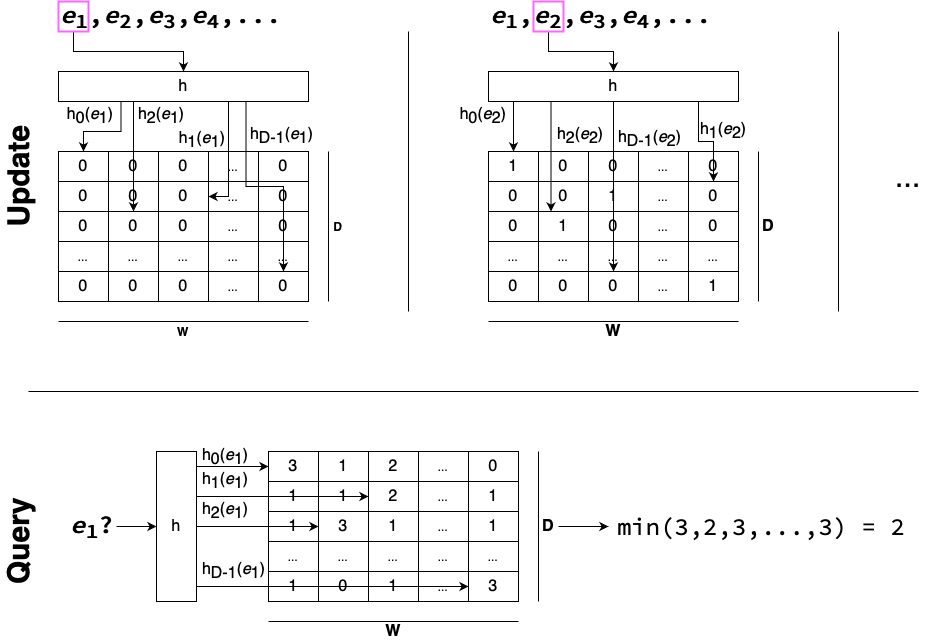
\includegraphics[width=0.9\textwidth]{figures/cm-example}
	\end{center}
	\caption{Example of a \cm sketch}\label{fig:countminexample}
\end{figure}

It is important to notice that the \cm might overestimate the frequency of an event due to hash collisions, since more than one event might be mapped to the same cell of the matrix. However, the pairwise independence requirement ensures that, for any row $i$ and any two distinct events $x\neq x'$,
\begin{equation*}
\prob[h_i(x)=h_i(x')] = \frac{1}{w},
\end{equation*}
with this probability being computed over all possible choices of the hash function.
Hence, by setting $w$ appropriately, we can control the expected number of collisions per row, and likewise, by choosing a sufficiently large $d$, we can control for the probability of having at least one row without collisions for a given event. In general, for two given parameters $\epsilon, \delta \in (0,1)$, by setting 
$w=O(2/\epsilon)$ and $d=O(\log1/\delta)$, we have
\begin{equation}
\label{eq:cm-prob}
\prob[C.\mathit{query}(x) - c(x) > \epsilon \|\strsetname{X}\|_1] < \delta,
\end{equation}
where $c(x)$ represents the true frequency of $x$, and $\|\strsetname{X}\|_1=\sum_{x_i}c(x_i)$ is the true total event count. Put another way, we can have the estimate error relative to the total event count to be `small' (no more than $\epsilon$) with `good' (at least $1-\delta$) probability.

\subsection{Using the \cm for counting \kmer{s}}
\label{subsec:cm-countingkmers}

Zhang \emph{et al.} proposed using a \cm sketch to count \kmer{s} \cite{Zhang2014}. Each \kmer is treated as an event, with reads being processed as a stream of \kmer{s}. The \kmer{s} can be hashed by interpreting them not as a string, but as a base-4 integer, with $\A=0$, $\C=1$, $\G=2$, $\T=3$. For example, the \kmer $\C\G\A\T\A$ can be interpreted as the integer $12030_{(4)} = 396_{(10)}$. Whenever we refer to hashing a \kmer, we use its integer interpretation. Using a \cm introduces the chance that any reported count will be an overestimate, the probability of which is approximately $(1-e^{-\frac{N}{w}})^d$, with $N$ the number of distinct \kmer{s} \cite{Zhang2014}.


Because the \kmer counts are used to determine if a \kmer should be added to the \dBG, as discussed in Section~\ref{subsec:dBG-selectingkmers}, a structure that can answer count queries can be extended to implement the membership query operation, with a \kmer $X$ being considered to be represented in the graph if $C.\mathit{query}(X).c \geq t$. 
Assuming that the vast majority of low-frequency \kmers occur no more than once or twice in the input reads, in order for such a \kmer to be unduly considered as real (false positive), its \cm estimate would have to be off by about $t$ or more. Because the \cm overestimation error is at most $\epsilon F$ with probability at least $1-\delta$, according to Eq~\ref{eq:cm-prob}, by controlling this maximum error to be at most $t$, we have that the expected false positive rate is no more than $\delta$. This amounts to setting the \cm dimensions to $w=O(2/\epsilon) = 2F/t$ and $d=1/\delta$.


%As the count returned by the \cm sketch can be overestimated by some error $\epsilon F$ with probability $\delta$ as established in Equation~\ref{eq:cm-prob}, we can arrive at an expression for the probability that a low-frequency \kmer will be considered to be a member of the \dBG by defining $\epsilon F = t$. This takes into account that most spurious \kmer{s} appear only once or twice in the reads, as discussed in Section~\ref{subsec:dBG-selectingkmers}. Due to the relationships between $w$ and $\epsilon$, and $d$ and $\delta$, we can decide the necessary size of the \cm sketch to achieve the desired false positive rate by making $\delta$ the desired rate, choosing $d = \log \frac{1}{\delta}$, and making $w = \frac{2}{\epsilon} = \frac{2F}{t}$.


% - Representation (what goes in each cell)
% - Operations:
%   - addOutEdge
%   - query 
% - Analysis space/time (may be done within previous sections)

% Because we expect each \kmer from the sequence to appear in the reads a number of times equals to the coverage, while spurious \kmer{s} will appear a low number of times \cite{Conway2011} \cite{Ghosh2019}, a structure used to count \kmer{s} (that implements the $\mathit{count}(x)$) can implement the membership query operation as $\mathit{memb}(x)=\mathit{count}(x) \geq t$. In this way, a \cm sketch can \toconsider{probabilistically} represent a \dBG with some false positive and false negative rates associated with the membership query operation. These rates can be controlled by $t$.\asq{Aqui talvez valha a pena falar que existem duas abordagens para tentar controlar as taxas de falsos positivos e negativos: 1. O valor de $t$ pode ser estabelecido, e, então, os valores de $w$ e $d$ são calculados de forma a minimizar a chance de um erro $\epsilon > t$; 2. Os valores $w$ e $d$ podem ser fixados, e, então, $t$ é decidido baseado nas estimativas esperadas para um \kmer espúrio \emph{vs.} um \kmer real.}

% Selecting the appropriate value for $t$ is not a trivial task, however, and is a trade-off between the false positive and false negative rates. Due to the fact that reads are generated randomly from the original genome, and that a number of real \kmer{s} will be replaced by spurious \kmer{s} because of sequencing errors, an universally optimal threshold \toconsider{that perfectly decides if a \kmer is spurious or not} does not exist. Higher values of $t$ are more likely to cut out spurious \kmer{s}, reducing false positive rates, but they also increase the chances of a real \kmer being missed, increasing false negative rates. Lower values of $t$ result in the opposite effect happening.

\subsection{\cm as a probabilistic NDS representation for \dBG{s}}
\label{subsubsec:cm-dbg}

Finally, in order to make the \cm more easily navigable, we expand the sketch such that each cell $C[i,j]$ in the matrix stores not only the counter $C[i,j].c$, but also a set of outedges $C[i,j].E$. The structure then provides an operation to \emph{update} the counters $C[i,h_i(X)].c$ associated with a given \kmer $X$ by one, and an operation to \emph{add an outedge} to the sets $C[i,h_i(X)].E$. The update operation is the same as in a regular \cm, and the procedure for adding an edge can be seen in Algorithm~\ref{alg:addOutEdge}.


\begin{algorithm}[htbp]
    \caption{$C.\mathit{add\_outedge}(X, a)$}\label{alg:addOutEdge}
    \Input{C, the \dBCM; $X$, the \kmer; $a \in \{\A, \C, \G, \T\}$, the outedge label}
    \For{$i \gets 0, \ldots, d-1$}{
      $C[i,h_i(X)].E \gets C[i,h_i(X)].E \cup \{a\}$\\
    }
\end{algorithm}

Besides the query operation, used for obtaining the count for a given \kmer $X$, done in the same way as in a regular \cm, the \dBCM must also implement an operation for retrieving the outedges for $X$. This new operation is presented in Algorithm~\ref{alg:dbcm-outedges}.

\begin{algorithm}
	\caption{$C.\mathit{outedges}(X)$}\label{alg:dbcm-outedges}
  \Input{$C$, the \dBCM; $X$, the \kmer}
  \Output{The outedge set $E$}
	$E \gets \{\A, \C, \G, \T\}$\\
	\For{$i = 1, \ldots, d$}{
		$E \gets E \cap C[i,h_i(X)].E$\\
	}
	\Return{$E$}
\end{algorithm}

In practice, due to a node having at most four outedges corresponding to the bases $\{\A, \C, \G, \T\}$, the set storing them can be represented with four bits indicating whether each of them is present. An edge is added by setting the corresponding bit, and the intersection is obtained by performing the bitwise AND operation. Moreover the set of outedges and the counter are packed together in a single 16-bit integer. This layout can be visualized in Figure~\ref{fig:dbcm-bit_use}. When using a $k$ such that $4^k > |S|$, then each \kmer in $S$ is expected to appear only once in $S$, and a number of times equals to the coverage $c$ in the reads. Considering that $c$ is not a very high value (commonly below $200$), each counter can be represented by a 12-bit integer, accounting for the expected count for all real \kmer{s}, as well as possible collisions.

\begin{figure}[htbp]
  \centering
  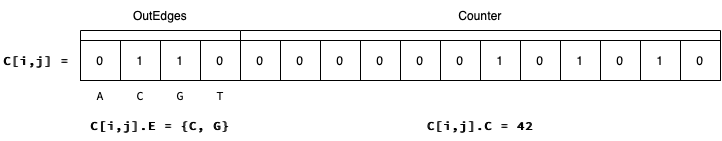
\includegraphics[width=0.9\textwidth]{figures/dbcm-bit_use}
  \caption{A \dBCM cell}\label{fig:dbcm-bit_use}
\end{figure}

\subsection{\dBCM Construction}
\label{subsubsec:dbcm-construction}

The \dBCM is constructed as the reads are processed by incrementing the counters for each \kmer as they are read. Once a \kmer{'s} counter reaches the threshold for presence $t$, an outedge is added from the \kmer that preceded it to itself. That is if \kmer{s} $X$ and $Y$ happen consecutively in a read, and $C.\mathit{query}(Y).c \geq t$, then the operation $C.\mathit{add\_outedge}(X, Y[k-1])$ is performed. 
%
By only adding the edge $X\stackrel{a}{\longrightarrow}Y$ when $Y$ is considered to be high-frequency we avoid adding edges to nodes that we do not yet know to exist. Such edges would point, in the best case, to a node that would not be found to be on the graph, resulting in unnecessary operations before the path is considered finished, and in the worst case would be interpreted, in a collision, as a diferent edge, resulting in a new branch on the graph. Conversely, the source node $X$ does not need to be considered present on the graph for the edge to be added. This avoids the scenario where both $X$ and $Y$ are real \kmer{s}, but $Y$ shows up for the last time before $X$ is considered to be present, in which case the edge would never be added. Moreover, adding an outedge to a \kmer that is not considered to be present in the graph is irrelevant, as the \kmer will be ignored during traversal. Because the resulting \dBCM is dependent on the threshold $t$ used during construction, we store this value and denote it by $C.t$.

Besides updating the \dBG represented by the \dBCM by counting the \kmer{s} and tracking the outedges, the construction step also generates a set of \kmer{s} known to be represented in the graph that can be used for traversal, as further discussed in Section~\ref{subsubsec:dbcm-navigation}. The procedure for constructing a \dBCM can be seen in Algorithm~\ref{alg:dbcm-construction}. Like Conway \& Bromage \cite{Conway2011}, we process each read in the forward and in the reverse complement direction, without merging \kmer{s} corresponding to reverse complements of each other.

\begin{algorithm}
	\caption{$C.\mathit{construct}(\readset, t, n)$}\label{alg:dbcm-construction}
  \Input{$C$, the \dBCM; $\readset$, the set of reads; $t$, the frequency threshold for a \kmer to be considered true; $n$, the number of \kmer{s} from each read to be included in \strsetname{S}}
  \Output{\strsetname{S} the set of starting \kmer{s}}
  $C.t \gets t$\\
  $\strsetname{S} \gets \emptyset$\\
  $\overline{\readset} \gets \{\overline{R}; R \in \readset \}$\Comment{The set of the reverse complements of the reads}\\
  \For{$R \in \readset \cup \overline{\readset}$}{
    $X \gets \varnothing$\\
    $i \gets 0$\\
    \For{$Y \in \kmer{s}(R)$}{
      $C.\mathit{update}(Y)$\\
      \If(\Comment{see Section~\ref{subsubsec:dbcm-operations}}){$C.\mathit{is\_member}(Y)$}{
        \If{$i \leq n$} {
          $\strsetname{S} \gets \strsetname{S} \cup \{Y\}$\\
        }
        \If{$i > 0$}{
          $C.\mathit{add\_outedge}(X, Y[i-1])$\\
        }
      }
      $i \gets i+1$\\
      $X \gets Y$\\
    }
  }
  \Return{\strsetname{S}}
\end{algorithm}

\subsection{\dBCM Operations}
\label{subsubsec:dbcm-operations}

We can implement the operations listed in Section~\ref{subsubsec:dbg-operations} using the \dBCM as follows.

\paragraph*{Membership query} Given the desired presence threshold $t$, we can implement the membership query operation in the \dBCM as $C.\mathit{is\_member}(X) \equiv C.\mathit{query}(X).c \geq C.t$.

\paragraph*{Forward neighbor query} $C.\mathit{forward\_neighbor}(X, a) \equiv a\in C.\mathit{query}(X).E$.

\paragraph*{Neighborhood query} We can transform the set of outedges $C[i,j].E$ into a set of \kmer{s} by extending the \kmer with the outedges from the set. As such, a procedure for generating the set of neighbors for a given \kmer $X$ is found in Algorithm~\ref{alg:dbcm-neighbors}.

\begin{algorithm}
	\caption{$C.\mathit{neighbors}(X)$}\label{alg:dbcm-neighbors}
  \Input{$C$, the \dBCM; $X$, a \kmer}
  \Output{$N$, a set of \kmer{s} that are neighbors of $X$}
  $N \gets \emptyset$\\
  \For{$a \in C.\mathit{query}(X).E$}{
    $N \gets N \cup \{X[1:k-1] \cdot a\}$\\
  }
	\Return{$N$}
\end{algorithm}

\subsection{\dBCM Traversal}
\label{subsubsec:dbcm-navigation}

This structure can be traversed in a breadth-first order from an initial set of \kmer{s} $\strsetname{S}$ by querying for their out-edges and then querying each of their neighbors, repeating this for each neighbor found to be in the graph. This procedure can be observed in Algorithm~\ref{alg:traversal}.

% \begin{algorithm}
% 	\caption{$C.\mathit{traverse}(\strsetname{S}, t)$}\label{alg:traversal}
%   \Input{$C$, the \dBCM; $\strsetname{S}$, the set of starting \kmer{s}; $t$, the threshold of presence}
%   \Output{$V$, the set of \kmer{s} queried from the \dBCM during traversal}
%   $F \gets$ empty Queue\\
%   \For{$s \in \strsetname{S}$}{
%     enqueue($F$, $s$)\\
%   }
%   $V \gets \{\}$\\
%   \While{$F$ is not empty} {
%     $u \gets$ dequeue($F$)\\
%     $V \gets V \cup \{u\}$\\
%     $n, E \gets C.query(u)$\\
%     \If{$n \geq t$}{
%       \For{$a \in E$}{
%         $v \gets$ extend($u$, $a$)\\
%         \If{$v \notin V$}{
%           enqueue($F$, $v$)\\
%         }
%       }
%     }
%   }
% 	\Return{$V$}
% \end{algorithm}

\begin{algorithm}
	\caption{$C.\mathit{traverse}(\strsetname{S}, t)$}\label{alg:traversal}
  \Input{$C$, the \dBCM; $\strsetname{S}$, the set of starting \kmer{s}; $t$, the threshold of presence}
  \Output{$V$, the set of \kmer{s} queried from the \dBCM during traversal}
  $F \gets$ empty Queue\\
  \For{$s \in \strsetname{S}$}{
    enqueue($F$, $s$)\\
  }
  $Q \gets \{\}$\\
  \While{$F$ is not empty} {
    $u \gets$ dequeue($F$)\\
    $Q \gets Q \cup \{u\}$\\
    \If{$C.\mathit{is\_member}(u, t)$}{
      \For{$v \in C.\mathit{neighbors}(u)$}{
        \If{$v \notin Q$}{
          enqueue($F$, $v$)\\
        }
      }
    }
  }
	\Return{$Q$}
\end{algorithm}

\paragraph*{Selecting the starting set $\strsetname{S}$ of \kmer{s} for traversal} Ideally, only the first \kmer from the original sequence $S$ is needed to perform the traversal of the grap, but unfortunately it is not possible to determine where in the original sequence a read was taken from. One option is to use all the \kmer{s} from the reads that are found to be in the graph, but we argue that this set is unnecessarily large. We can instead reduce the size of $\strsetname{S}$ by only considering the \kmer{s} that are at the start of their reads since the following \kmers would be reachable from it anyway.

\section{The \dB Hashtable}
\label{sec:debruijnhashtable}
% - Structure
%   - fingerprint
%   - Outedges
% - Hash function 
% - Collision resolution
% - Operations 
%   - Add node/edge
%   - Query node/edge/star 
% - Analysis 

We also propose a new hashtable-based representation for the \dBG, called \keyterm{\dB Hashtable} \dBHT, that is made more space-efficient by not storing the \kmer directly. Instead, the slot $T[i]$ containing the \kmer $X$ stores a \keyterm{fingerprint} $T[i].f = f_X$, computed from $X$ as described in Section~\ref{sec:fingerprint}, along with the set of outgoing edges from $X$, $T[i].E$,  as described in Section~\ref{sec:debruijncountmin}.

When inserting a \kmer $X$ into a \dBHT of capacity $m$, a hash value $h_X$ and the fingerprint $f_X$ are calculated in parallel. The hash value, computed as described in Section~\ref{sec:fibhash}, determines the initial position $p_0$ in which the \kmer should be stored. If this slot is empty, then the fingerprint is written there. Otherwise, collisions are resolved by linear probing, that is the subsequent positions $(p_0+j)\mod m$, for $j=0\ldots m-1$, are checked until a free slot is found. If, however, a slot containing $f_X$ is found before, then $X$ is considered to be already represented in $H$ and the insertion aborts. This process is detailed in Algorithm~\ref{alg:ht-insert}. 
Notice that this requires always having some unused slots, that is, having a \emph{load factor} $0 < \alpha=n/m < 1$, where $n$ is the number of used positions. Higher values of $\alpha$ will result in higher space-efficiency, but also` more collisions. Lower values have the opposite effect. 


\begin{algorithm}
	\caption{$T.\mathit{insert}(X$)}\label{alg:ht-insert}
	\Input{$T$: a \dBHT with capacity $m$; $X$: the \kmer to be inserted}
	$h_X \gets \mathit{fibhash}(X, m)$\Comment{see Section~\ref{sec:fibhash}}\\
	$f_X \gets \mathit{fingerprint}(X)$\Comment{see Section~\ref{sec:fingerprint}}\\
	$i \gets h_X$\\
	\While{$T[i]$ is not empty}{
		\eIf{$T[i].f = f_X$}{
			\Return{}\Comment{$X$ already in $T$}
		}{
			$i \gets (i + 1)\mod m$\\
		}
	}
	$T[i].f\gets f_X$\\
	$T[i].E\gets \varnothing$\\
\end{algorithm}

To query the hashtable for a \kmer/node $X$, the same sequence of positions as in the insertion are probed until the desired fingerprint $f_X$ is found, or a free position is reached, in which case we can conclude that the \kmer is absent from the structure. This operation is presented in Algorithm \ref{alg:ht-query}.

\begin{algorithm}
	\caption{$T.\mathit{query}(X)$}\label{alg:ht-query}
  \Input{$T$: a \dBHT with capacity $m$; $X$: the \kmer to be queried}
	$h_X \gets \mathit{fibhash}(X, m)$\\
  $f_X \gets \mathit{fingerprint}(X)$\\
	$i \gets h_X$\\
	\While{$T[i]$ is not empty}{
    \eIf{$T[i].f = f_X$}{
      \Return{$T[i].E$}
    }{
		  $i \gets (i + 1) \mod m$\\
    }
	}
  \Return{$\varnothing$}
\end{algorithm}


Adding an edge $X\stackrel{a}{\longrightarrow}Y$ to the \dBHT is similar to adding a \kmer node, and breaks down to, first, locating the slot $T[i]$ of the source node $X$, and then adding the corresponding edge label $a$ to its set of outedges. As before, this is done by setting the appropriate bit of the  4-bit pattern $T[i].E$. This procedure is detailed in Algorithm~\ref{alg:ht-addedge}. Note that, because two \kmer{s} can be mapped to the same cell, the outedges stored for both of them will be the same and will contain the true outedges of each one individually. This further makes it important that edges only be added to nodes known to be in the graph, which the \dBHT does not verify.


\begin{algorithm}
  \caption{$T.\mathit{add\_outedge}(X, a)$}\label{alg:ht-addedge}
  \Input{$T$: a \dBHT with capacity $m$; $X \in \{\A, \C, \G, \T\}^k$: the \kmer to be queried; $a \in \{\A, \C, \G, \T\}$: the edge label to be added}
  $h_X \gets \mathit{fibhash}(X, m)$\\
  $f_X \gets \mathit{fingerprint}(X)$\\
  $i \gets h_X$\\
  \While{$T[i]$ is not empty}{
    \eIf{$T[i].f = f_X$}{
      $T[i].E \gets T[i].E \cup \{a\}$\\
    }{
      $i \gets (i + 1) \mod m$\\
    }
  }
\end{algorithm}


\subsection{Modular Fibonacci Hashing}\label{sec:fibhash}

The \dBHT uses the Fibonacci hashing algorithm \cite{Skarupke2018} to hash the \kmers, which leverages the property of the golden ratio $\phi$ that, given a range $r$, the set $\Gamma = \{i\cdot \frac{r}{\phi} \mod r ;\ i \in \mathbb{N}\}$ is evenly distributed over $r$, and has no period. Note that the modulo operator here means the remainder of a real division, so that the elements of $\Gamma$ are real numbers. The integer hashing algorithm that maps a number to the range $[0, m]$ works by multiplying the key $X$ by the closest integer to the value $m/\phi$ taking the result modulo $m$. The $\mathit{fibhash}$ function can be seen in Algorithm~\ref{alg:fibonacci-hash}.

\begin{algorithm}
  \caption{$\mathit{fibhash}(X, m)$}\label{alg:fibonacci-hash}
  \Input{$X$, the key to be hashed; $m$, the range into which it should be hashed}
  \Return{$(\mathit{round}({m/\phi})\cdot X) \mod m$}
\end{algorithm}

\subsection{\kmer Fingerprinting}\label{sec:fingerprint}

We obtain a 3-bit fingerprint of a \kmer by performing a modified version of the Fibonacci hashing algorithm. We use the hashing function described above for the range addressable by a 64-bit integer ($r=2^{64}$), with the modulo operation being performed implicitly by using integer multiplication with a 64-bit int type. Then we take the three most significant bits of the result as the fingerprint. We choose the most significant bits because, as observed by Skarupke, they present the best avalanche behavior, i.e. flipping any one bit individually from the input causes each bit in the output to flip with close to 50\% probability \cite{Skarupke2018}. In practice this procedure, shown in Algorithm~\ref{alg:fingerprint}, is very fast due to it foregoing the modulo operation and performing only one multiplication by a constant and a bitwise shift operation to extract the most significant bits. Note that, although $11400714819323198486$ is actually closer to $2^{64}/\phi$, we prefer an odd number so as not to waste the last bit.

\begin{algorithm}
  \caption{$\mathit{fingerprint(X)}$}\label{alg:fingerprint}
  \Input{$X$, the key to fingerprint}
  Let $\psi$ be the 64-bit constant $\mathit{round}({2^{64}}/{\phi})=11400714819323198485$\\
  \Return{$(X \cdot \psi ) >> 61$}
 
\end{algorithm}

\subsection{\dBHT Construction}
\label{subsubsec:dbht-construction}

We construct the \dBHT by traversing the \dBCM representation of the graph starting from the set of initial nodes $\strsetname{S}$, which we insert into the \dBHT, then inserting all of their true neighbors via the corresponding outedges, and then repeating the process from those neighbors. This procedure can be seen in Algorithm~\ref{alg:dbht-construct}.

\begin{algorithm}
	\caption{$T.\mathit{construct}(C)$}\label{alg:dbht-construct}
  \Input{$T$, the \dBHT; $C$, a \dBCM; $t$, the frequency threshold for a \kmer to be considered to be represented in $C$}
  $F \gets$ empty Queue\\
  \For{$s \in \strsetname{S}$}{
    enqueue($F$, $s$)\\
  }
  $Q \gets \{\}$\\
  \While{$F$ is not empty} {
    $u \gets$ dequeue($F$)\\
    $Q \gets Q \cup \{u\}$\\
    \If{$C.\mathit{is\_member}(u, t)$}{
      $T.\mathit{insert}(u)$\\
      \For{$v \in C.\mathit{neighbors}(u)$}{
        \If{$C.\mathit{is\_member}(v, t)$}{
          $T.\mathit{add\_outedge}(u, v[k-1])$\\
          \If{$v \notin Q$}{
            enqueue($F$, $v$)\\
          }
        }
      }
    }
  }
\end{algorithm}

\subsection{\dBHT Operations}

\paragraph*{Membership query} The membership query is just the evaluation of if the query operation found the \kmer: $T.\mathit{is\_member}(X) \equiv T.\mathit{query}(X) \neq \varnothing$.

\paragraph*{Forward neighbor query} As in the \dBCM, the forward neighbor query just checks if the given base $a$ is in the set of outedges of $X$: $T.\mathit{forward\_neighbor}(X, a) \equiv a \in T.\mathit{query}(X)$.

\paragraph*{Neighborhood query} Again, similarly to the \dBCM, the neighbors of $X$ can be obtained by extending it with its outedges, as presented in Algorithm~\ref{alg:dbht-neighbors}.

\begin{algorithm}
	\caption{$T.\mathit{neighbors}(X)$}\label{alg:dbht-neighbors}
  \Input{$T$, the \dBHT; $X$, a \kmer}
  \Output{$N$, a set of \kmer{s} that are neighbors of $X$}
  $N \gets \emptyset$\\
  \For{$a \in T.\mathit{query}(X)$}{
    $N \gets N \cup \{X[1:k-1] \cdot a\}$\\
  }
	\Return{$N$}
\end{algorithm}

\subsection{\dBHT Traversal}

We traverse \dBHT in a breadth-first manner from a starting set of \kmer{s} \strsetname{S} by adding them to a queue. Then we dequeue one node and query for its neighbors, adding them to the queue if they weren't visited yet. We repeat this process until the queue is empty. This procedure can be seen in Algorithm~\ref{alg:dbht-navigate}. As in the traversal of the \dBCM, the result is the set of \kmer{s} that were queried during traversal.

\begin{algorithm}
	\caption{$T.\mathit{traverse}(\strsetname{S}, t)$}\label{alg:dbht-navigate}
  \Input{$C$, the \dBCM; $\strsetname{S}$, the set of starting \kmer{s}}
  \Output{$V$, the set of \kmer{s} queried from the \dBCM during traversal}
  $F \gets$ empty Queue\\
  \For{$s \in \strsetname{S}$}{
    enqueue($F$, $s$)\\
  }
  $Q \gets \{\}$\\
  \While{$F$ is not empty} {
    $u \gets$ dequeue($F$)\\
    $Q \gets Q \cup \{u\}$\\
    \If{$C.\mathit{is\_member}(u)$}{
      \For{$v \in C.\mathit{neighbors}(u)$}{
        \If{$v \notin Q$}{
          enqueue($F$, $v$)\\
        }
      }
    }
  }
	\Return{$Q$}
\end{algorithm}